\documentclass{beamer}
\usetheme{Berlin}

\title{Refresher On Scientific Programming With Python for Engineers}
\subtitle{Course: Complex Systems Modeling}
\author{Robert Flassig}
\institute{Brandenburg University of Applied Sciences}
\date{\today}

\usepackage{tikz}
\usetikzlibrary{decorations.pathmorphing}

\begin{document}
\begin{frame}
\titlepage
\end{frame}

\begin{frame}
\frametitle{Outline}
\tableofcontents
\end{frame}

\section{Python Basics Refresher}

\subsubsection*{Introduction to Python}

\begin{frame}[fragile]
\frametitle{Introduction to Python}
\begin{itemize}
    \item Python is an easy-to-learn, versatile programming language widely used in scientific computing, data analysis, web development, and more.
    \item Python code is known for its readability and simplicity.
    \item Python uses indentation to define code blocks (e.g., loops, functions).
\end{itemize}

\begin{block}{Example of Python Code}
\begin{verbatim}
# This is a comment
print("Hello, world!")  # Output: Hello, world!
\end{verbatim}
\end{block}
\end{frame}

\subsubsection*{Variables and Data Types}

\begin{frame}
\frametitle{Variables and Data Types (1/2)}
\begin{itemize}
    \item \textbf{Variables} store values and are created upon assignment. No need to declare types explicitly.
    \item Common \textbf{Data Types} in Python:
    \begin{itemize}
        \item \texttt{int} - Integer numbers (e.g., \texttt{42})
        \item \texttt{float} - Floating-point numbers (e.g., \texttt{3.14})
        \item \texttt{str} - Strings (e.g., \texttt{"Hello"})
        \item \texttt{bool} - Boolean values (\texttt{True} or \texttt{False})
    \end{itemize}
\end{itemize}

\end{frame}

\begin{frame}[fragile]
\frametitle{Variables and Data Types (2/2)}
\begin{block}{Example of Python Code}
\begin{verbatim}
# Variable assignment
x = 10        # int
y = 3.14      # float
name = "Alice"  # str
is_student = True  # bool
\end{verbatim}
\end{block}
\end{frame}


\subsubsection*{Basic Operations}

\begin{frame}[fragile]
\frametitle{Basic Operations}
\begin{itemize}
    \item Python supports basic arithmetic and logical operations:
    \begin{itemize}
        \item \textbf{Arithmetic:} \texttt{+}, \texttt{-}, \texttt{*}, \texttt{/}, \texttt{**} (exponent), \texttt{\%} (modulus)
        \item \textbf{Logical:} \texttt{and}, \texttt{or}, \texttt{not}
    \end{itemize}
\end{itemize}
\tiny{
\begin{block}{Example of Python Code}
\begin{verbatim}
# Arithmetic operations
a = 10 + 5   # Addition: 15
b = 7 - 3    # Subtraction: 4
c = 6 * 2    # Multiplication: 12
d = 8 / 4    # Division: 2.0
e = 5 ** 2   # Exponentiation: 25
f = 10 % 3   # Modulus: 1

# Logical operations
is_even = (a % 2 == 0)  # False
is_positive = (b > 0) and (c > 0)  # True
\end{verbatim}
\end{block}}
\end{frame}

\subsubsection*{Control Flow: Conditionals}

\begin{frame}[fragile]
\frametitle{Control Flow: Conditionals}
\begin{itemize}
    \item Use \texttt{if}, \texttt{elif}, and \texttt{else} statements to control the flow of your program.
    \item Indentation is crucial in Python; it defines the block of code that belongs to each conditional.
\end{itemize}
\tiny{
\begin{block}{Example of Python Code}
\begin{verbatim}
# Conditional statements
number = 10

if number > 0:
    print("Positive")
elif number == 0:
    print("Zero")
else:
    print("Negative")
\end{verbatim}
\end{block}}
\end{frame}

\subsubsection*{Loops: \texttt{for} and \texttt{while}}

\begin{frame}[fragile]
\frametitle{Loops: \texttt{for} and \texttt{while}}
\begin{itemize}
    \item Use \texttt{for} loops to iterate over a sequence (e.g., list, range).
    \item Use \texttt{while} loops to repeat a block of code as long as a condition is \texttt{True}.
\end{itemize}
\tiny{
\begin{block}{Example of Python Code}
\begin{verbatim}
# for loop
for i in range(5):
    print(i)  # Output: 0 1 2 3 4

# while loop
count = 0
while count < 5:
    print(count)
    count += 1  # Output: 0 1 2 3 4
\end{verbatim}
\end{block}}
\end{frame}

\subsubsection*{Functions}

\begin{frame}[fragile]
\frametitle{Functions}
\begin{itemize}
    \item Functions allow you to organize code into reusable blocks.
    \item Define a function using the \texttt{def} keyword followed by the function name and parameters.
\end{itemize}
\tiny{
\begin{block}{Example of Python Code}
\begin{verbatim}
# Defining a function
def greet(name):
    return "Hello, " + name

# Calling the function
message = greet("Alice")
print(message)  # Output: Hello, Alice
\end{verbatim}
\end{block}}
\end{frame}

\subsubsection*{Working with Matplotlib}

\begin{frame}[fragile]
\frametitle{Working with Matplotlib}
\begin{itemize}
    \item \texttt{matplotlib} is a popular library for creating static, animated, and interactive visualizations in Python.
    \item To install \texttt{matplotlib}, use: \texttt{!pip install matplotlib}.
    \item Commonly used to create plots, charts, and other graphical representations.
\end{itemize}
\tiny{
\begin{block}{Example of Python Code}
\begin{verbatim}
import matplotlib.pyplot as plt

# Data for plotting
x = [1, 2, 3, 4, 5]
y = [10, 15, 13, 17, 14]

# Creating a simple plot
plt.plot(x, y, marker='o')
plt.title('Simple Line Plot')
plt.xlabel('X-axis')
plt.ylabel('Y-axis')
plt.show()
\end{verbatim}
\end{block}}
\end{frame}

\subsubsection*{Programming Exercises}

\begin{frame}
\frametitle{Programming Exercises}
\begin{itemize}
    \item \textbf{Exercise 1: Basic Arithmetic Operations}
    \begin{itemize}
        \item Write a function that takes two numbers as inputs and returns their sum, difference, product, and quotient.
    \end{itemize}

    \item \textbf{Exercise 2: Plotting with Matplotlib}
    \begin{itemize}
        \item Use \texttt{matplotlib} to create a bar chart showing the population of five cities.
        \item Customize the chart with labels, title, and different colors for each bar.
    \end{itemize}

    \item \textbf{Exercise 3: Generating the Sierpinski Carpet}
    \begin{itemize}
        \item Write a recursive function to generate an image of the Sierpinski carpet.
        \item Use \texttt{matplotlib} to visualize the fractal pattern.
    \end{itemize}
\end{itemize}
\end{frame}

\section{How to Model the Sierpinski Carpet}
% Frame 1: How to Model the Sierpinski Carpet
\begin{frame}{How to Model the Sierpinski Carpet}
    \begin{itemize}
        \item \textbf{Understanding the Sierpinski Carpet:}
        \begin{itemize}
            \item A fractal pattern formed by recursively subdividing a square into 9 smaller squares.
            \item Remove the central square in each step.
        \end{itemize}
        \item \textbf{Steps to Construct:}
        \begin{enumerate}
            \item \textbf{Base Case:} Start with a single square.
            \item \textbf{Recursion:} Divide each square into 9 parts, remove the center.
            \item \textbf{Repeat:} Apply recursively to remaining 8 squares.
        \end{enumerate}
        \item \textbf{Key Concepts:} Fractals, recursion.
    \end{itemize}
\end{frame}

% Frame 2: Implementing the Sierpinski Carpet in Python
\begin{frame}{Implementing the Sierpinski Carpet in Python}
    \begin{itemize}
        \item \textbf{Using Recursion:} Define a function for square position, size, and depth.
        \item \textbf{Libraries:} Use \texttt{matplotlib} for visualization.
        \item \textbf{Pseudocode:}
        \begin{enumerate}
            \item \textbf{Base Case:} If depth is 0, draw a filled square.
            \item \textbf{Recursive Case:} Divide current square into 9 parts. Recursively draw the 8 outer squares.
        \end{enumerate}
        \item \textbf{Code Structure:} 
        \begin{itemize}
            \item Define a \texttt{draw\_square} function for drawing.
            \item Loop for positioning smaller squares.
        \end{itemize}
        \item \textbf{Tip:} Limit recursion depth to manage computation.
    \end{itemize}
\end{frame}

% Frame 3: Minimal Python Code for Sierpinski Carpet
\begin{frame}[fragile]{Minimal Python Code for Sierpinski Carpet}
\tiny{
    \begin{block}{Python Code}
    \begin{verbatim}
import matplotlib.pyplot as plt

def draw_carpet(x, y, size, depth):
    if depth == 0:
        plt.gca().add_patch(plt.Rectangle((x, y), size, size, color='black'))
    else:
        new_size = size / 3
        for i in range(3):
            for j in range(3):
                if i != 1 or j != 1:  # Skip the center square
                    draw_carpet(x + i * new_size, y + j * new_size, new_size, depth - 1)

plt.figure(figsize=(6, 6))
draw_carpet(0, 0, 1, 4)  # Adjust depth as needed
plt.gca().set_aspect('equal')
plt.axis('off')
plt.show()
    \end{verbatim}
    \end{block}
    \begin{itemize}
        \item \textbf{Explanation:} Recursively divides the square into smaller squares and skips the center.
        \item \textbf{Adjustments:} Modify the depth parameter for different levels of detail.
    \end{itemize}}
\end{frame}

\section{Modeling Oscillators}

\begin{frame}{Introduction to the Harmonic Oscillator}
    \begin{itemize}
        \item The harmonic oscillator is a fundamental model in physics and engineering.
        \item It describes a mass-spring system where the restoring force is proportional to displacement.
        \item Real-world examples:
        \begin{itemize}
            \item Car suspension systems.
            \item Building structures during earthquakes.
            \item Vibrations in mechanical components.
        \end{itemize}
    \end{itemize}
\end{frame}

\begin{frame}{Harmonic Oscillator: Mass-Spring System}
    \begin{center}
    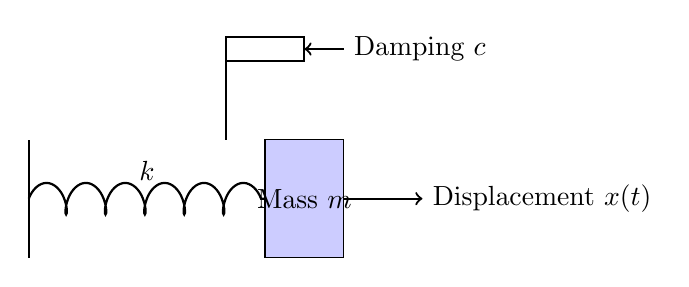
\begin{tikzpicture}
        % Draw the mass
        \filldraw[fill=blue!20] (3,0) rectangle (4,1.5) node[pos=.5] {Mass $m$};

        % Draw the spring
        \draw[thick, decorate, decoration={coil, aspect=0.5, segment length=5mm, amplitude=2mm}] (0,0.75) -- (3,0.75);
        
        % Draw the wall
        \draw[thick] (0,0) -- (0,1.5);
        
        % Label the spring
        \node at (1.5, 1.1) {$k$};
        
        % Label the damping
        \draw[->, thick] (4, 0.75) -- (5, 0.75) node[right] {Displacement $x(t)$};
        
        % Damping element
        \draw[thick] (2.5, 1.5) -- (2.5, 2.5);
        \draw[thick] (2.8, 2.5) -- (3.2, 2.5);
        \draw[thick] (2.5, 2.5) rectangle (3.5, 2.8);
        \draw[thick, <-] (3.5, 2.65) -- (4, 2.65) node[right] {Damping $c$};
    \end{tikzpicture}
    \end{center}
\end{frame}

\begin{frame}{Modeling Task: Real-World to Equations}
    \begin{itemize}
        \item \textbf{Objective:} Model the motion of the mass attached to a spring with damping.
        \item \textbf{Assumptions:}
        \begin{itemize}
            \item The spring follows Hooke's law: $F_s = -kx$.
            \item The damping force is proportional to velocity: $F_d = -c\dot{x}$.
        \end{itemize}
        \item \textbf{Newton's Second Law:} The sum of forces on the mass equals mass times acceleration:
        \[
        m \ddot{x}(t) = -kx(t) - c \dot{x}(t).
        \]
        \item \textbf{Resulting Differential Equation:}
        \[
        m \ddot{x}(t) + c \dot{x}(t) + k x(t) = 0.
        \]
    \end{itemize}
\end{frame}

\begin{frame}{Equations of Motion: Damped Harmonic Oscillator}
    \begin{itemize}
        \item The system can be described by the second-order linear differential equation:
        \[
        m \ddot{x}(t) + c \dot{x}(t) + k x(t) = 0.
        \]
        \item \textbf{Parameters:}
        \begin{itemize}
            \item $m$: Mass of the object (kg).
            \item $c$: Damping coefficient (kg/s).
            \item $k$: Spring constant (N/m).
        \end{itemize}
        \item \textbf{Special Cases:}
        \begin{itemize}
            \item \textit{Undamped Oscillator}: $c = 0$, simple harmonic motion.
            \item \textit{Overdamped, Critically Damped, Underdamped}: Different behaviors based on $c^2 - 4mk$.
        \end{itemize}
    \end{itemize}
\end{frame}

\begin{frame}{Numerical Simulation and Animation}
    \begin{itemize}
        \item Numerical methods, such as Euler's method, can be used to approximate the solution.
        \item We can visualize the motion of the oscillator by plotting position $x(t)$ over time.
        \item We can also visualize the phase space $x(t)$ vs. $\dot{x}(t)$.
        \item Let's explore the Python code to simulate and animate this system.
    \end{itemize}
\end{frame}


\end{document}